\ifx\wholebook\relax \else

\documentclass{article}

\input{../common-zh-cn.tex}

\setcounter{page}{1}

\begin{document}

\title{群、环、域}

\author{刘新宇
\thanks{{\bfseries 刘新宇} \newline
  Email: liuxinyu95@gmail.com \newline}
  }

\maketitle
\fi

\markboth{群、环、域}{编程的数学原理}

\ifx\wholebook\relax
\chapter{群、环、域}
\numberwithin{Exercise}{chapter}
\fi

\epigraph{你只要能把自己提出的那些“点、线、面”都说的跟“桌子、椅子、啤酒杯子”一样自然连贯就行。}{——大卫$\cdot$希尔伯特}

\begin{wrapfigure}{R}{0.3\textwidth}
 \centering
 \includegraphics[scale=0.35]{img/Escher-Liberation-1955.eps}
 \captionsetup{labelformat=empty}
 \caption{艾舍尔《解放》}
 \label{fig:clay-token}
\end{wrapfigure}

我们人类在长期的生产生活中逐渐养成了对事物分类整理的习惯。不同但相近的东西被归为一类。对整个类适用的性质和方法,对类中的不同事物都有效。这样我们就从解决具体的单一的问题,提高到一下子解决整类的抽象的问题,极大地丰富了我们认识掌握世界的能力。

在第一章中,我们曾经从自然数的累加和阶乘中归纳抽象出了“叠加”操作。我们观察它们相似的结构,将累加中的0和阶乘中的1抽象成单位元,将累加中的加法和阶乘中的乘法抽象成某种二元运算,这样就在更高的层次抽象出了自然数的叠加。进而可以用这一抽象的叠加操作解决诸如斐波那契数列这样的一大类和自然数同构的问题。

再举一个例子。我们在第一章中,还定义了列表上的抽象叠加操作$foldr$。可以利用这个抽象工具把一列数累加起来:$sum = foldr(0, +)$,也可以把一列数乘到一起:$product = foldr(1, \times)$。在计算机程序中,人们可以定义一种叫做“二叉搜索树”的数据结构。第二章中,我们曾经介绍过二叉树的定义。二叉搜索树是一种特殊的二叉树,它要求树中元素的类型A是可以比较的\footnote{这里比较的含义是抽象的,例如可以比大小,也可以是比较单词在字典中的先后顺序},并且对于任意分支节点,节点左侧子树中的所有元素都在此节点的元素之前,而右子树中的所有元素都在此元素之后。对排序二叉树,我们可以定义一个插入操作:

\[
\begin{array}{rcl}
  insert(nil, x) & = & node(nil, x, nil) \\
  insert(node(l, y, r), x) & = & \left.
  \begin{cases}
  x < y\ : & node(insert(l, x), y, r) \\
  x > y\ : & node(l, y, insert(r, x))
  \end{cases} \right.
\end{array}
\label{eq:BST-insert}
\]

根据这一定义,将一个元素$x$插入到二叉搜索树时,如果树为空,则结果为一个$node(nil, x, nil)$;否则,需要进一步比较$x$和分支节点中的元素$y$,如果$x$在前(用小于号代表),则递归地插入到左子树,否则地归地插入到右子树。联想累加和阶乘,插入操作和它们有什么相似之处呢?插入也是一个二元操作,而nil相当于单位元。这样我们就可以用抽象的叠加操作,将一列数字变成一棵搜索树:

\[
build = foldr(nil, insert)
\]

图\ref{fig:bst-example}展示了计算$build\ [4, 3, 1, 8, 2, 16, 10, 7, 14, 9]$产生的一棵二叉搜索树。

\begin{figure}[htbp]
  \centering
  \includegraphics[scale=0.5]{img/bst-example.ps}
  \caption{通过叠加产生的二叉搜索树}
  \label{fig:bst-example}
\end{figure}

我们人类对加法的认识也经历了类似的过程,最初的加法是针对具体事物的,例如采集的果实或者猎物。然后逐渐将具体事物的意义去除变成了针对抽象整数的加法。后来对数的认识扩充到了分数,虽然分数的具体相加过程和整数大相径庭,需要先对分母进行通分,然后将分子按照整数的法则相加,最后再进行约分。但是我们进一步将这两种不同的操作抽象成了有理数上的加法,人们深入思考它们的本质和性质,在每一次扩充数的认识时,都重新定义更加抽象的加法。从而有了实数上,复数上的加法。人们发现,对去除了具体意义的抽象事物成立的方法具备更大的应用范围。抽象方法能解决一类问题,而不是单一问题。计算机编程中逐渐发展出的面向对象方法,带泛型的类型系统,和动态类型系统都是某种意义上对抽象的一种支持机制。

在发展抽象的方法和工具时,必须时刻关注一个问题:“某一种抽象的适用范围有多大?什么情况下这一抽象会失效?”如果忽略了这一点,就会产生令人啼笑皆非的结果。比如人们总结抽象出了无穷几何级数的累加公式:$1 + x + x^2 + x^3 + ... = 1/(1-x)$。并用它成功解决了芝诺悖论\footnote{古希腊哲学家芝诺提出了四个著名的悖论,这里是指阿基里斯与乌龟悖论。阿基里斯是古希腊著名的英雄。芝诺假设阿基里斯追赶前面的乌龟,当他跑到乌龟出发的位置时,乌龟已经向前移动了一小段距离。阿基里斯必须继续跑到乌龟的新位置,但是此时乌龟又向前移动了。重复这一过程,芝诺认为阿基里斯永远赶不上乌龟。本书在第六章详细解释芝诺悖论。}。但是17世纪的数学家们把-1代入这个公式得到了$1 - 1 + 1 - 1 + ... = 1/2$这样的结果。这时有人提出了不同的意见:$S = (1 - 1) + (1 - 1)+ ... = 0$;还有人认为:$S = 1 + (-1 + 1) + (-1 + 1) + ... = 1$。有人赞同1/2的结果,因为$S = 1 - (1 - 1 + 1 - 1 + ...) = 1 -S$,解方程得$S = 1/2$。意大利数学教授格兰迪(1671 - 1742)还发现了更令人吃惊的结论。通过无穷级数:

\[
\begin{array}{l}
\dfrac{1}{1 + x + x^2} = 1 - x + x^3 - x^4 + x^6 - x^7 + ... \\[2ex]
\dfrac{1}{1 + x + x^2 + x^3} = 1 - x + x^4 - x^5 + x^8 - x^9 + ... \\
...
\end{array}
\]

令$x = 1$,可以得到无穷级数$1 - 1 + 1 - 1 + 1 - 1 + ...$的和可以等于1/3, 1/4, ...就连大数学家莱布尼茨也主张,它的和可能是0或者1,而且概率相等,所以其“真”值应该是它们的平均值1/2。格兰迪还做出了另一个“奇妙”的解释:父亲留给两个儿子一块宝石,由兄弟二人轮流保存,每人一年。于是,交给对方保存的时候,可以说所有权是0,自己保存的时候,可以说所有权是1,而平均而言,每人的所有权为1/2\cite{HanXueTao16}。这些奇怪的问题,要等到法国数学家柯西引入无穷级数收敛性后才得以解决。

编程中也有类似的问题。有一次在编写“自然归并排序”的算法时\footnote{自然归并排序是一种把一组元素按照大小顺序排列好的方法。它首先将元素分成若干组,每组中的元素顺序已经排好了。然后不断将这些组合并直到最后全部排好序。详细可参考\cite{LiuXinyu2017},第368页。},我需要将一列元素分成从大到小的若干组,例如把序列\texttt{[15, 9, 0, 12, 11, 7, 10, 5, 6, 13, 1, 4, 8, 3, 14, 2]}分组成\texttt{[[15, 9, 0], [12, 11, 7], [10, 5], [6], [13, 1], [4], [8, 3], [14, 2]]}。我知道标准库中提供了一个抽象工具\texttt{groupBy},它可以根据一个定义好的条件完成分组,例如:\texttt{groupBy (==) "Mississippi"}会得到结果\texttt{["M", "i", "ss", "i", "ss", "i", "pp", "i"]}。这样连续相等的元素就被分在一组。然而当我把大于等于作为分组条件,却得到了一个不正确的结果。\texttt{groupBy (>=) [15, 9, 0, 12, 11, 7, 10, 5, 6, 13, 1, 4, 8, 3, 14, 2]}产生的结果是\texttt{[[15, 9, 0, 12, 11, 7, 10, 5, 6, 13, 1, 4, 8, 3, 14, 2]]}。经过分析,原来\texttt{groupBy}是通过\texttt{span}实现的:

\lstset{language=Haskell, frame=single}
\begin{lstlisting}
groupBy _  []      = []
groupBy eq (x:xs)  = (x:ys) : groupBy eq zs
    where (ys, zs) = span (eq x) xs

span _ []        = ([], [])
span p xs@(x:xs')
     | p x       = let (ys, zs) = span p xs' in (x:ys, zs)
     | otherwise = ([], xs)
\end{lstlisting}

这样\texttt{span}就会连续判断15是否大于等于下一个元素,由于15恰好是整个列表中最大的,所以全部被归为了一组。实际上\texttt{groupBy}接受的分组条件是一个“抽象的相等”,它必须满足三个性质:自反性、对称性、和传递性:

\begin{itemize}
\item 自反性。$x = x$,即任何元素和它自己相等;
\item 对称性。若$x = y$,则$y = x$,即比较的顺序不影响结果。
\item 传递性。若$x = y$并且$y = z$,则$x = z$,如果两个元素相等,并且其中的一个和第三个元素相等,则这三个元素相等;
\end{itemize}

当对列表“Mississippi”使用等号作为条件分组时,三个条件都被满足,产生了正确的结果。但当将大于等于号($\geq$)作为“相等”条件传入时,就违反了自反性和对称性。这就是得到错误结果的原因。

本章我们介绍一些抽象的代数结构,它们不仅仅是对数的抽象,而且是对事物的概念、性质和关系的抽象。是很多伟大的思想和心智的结晶。

\section{群}

提到群论,就不得不提人类解方程的历史。方程是我们祖先发展出的一个强大工具。人们从古埃及的纸草书和古巴比伦的泥板书中发现,这些古代文明已经掌握了一元一次和二次方程的解法。但是一般三次方程的解法却一直没有进展。到了16世纪,经过意大利数学家们的努力,终于得到了一般三次方程和四次方程的根式解。最终卡尔丹在他的著作《大术》中总结人类历史上这千余年的结果。这些进展并不仅仅是未知数次数的提升,我们对数还有了全新的认识。早期二次方程的负根都被舍弃了,人们认为负数没有意义。不仅如此,人们认为方程的系数也必须是正数,在我们今天看来普通的方程$x^2 - 7x + 8 = 0$,必须用$x^2 + 8 = 7x$的形式来处理。在《大术》中,卡尔丹列出了20种不同类型的四次方程,他说还有67种其它类型的四次方程没有给出,原因仅仅是因为四次方程各项的系数可以为负数和零\cite{HanXueTao2012}。直到法国数学家韦达才将方程的形式统一。在解方程时,负数的根式一直被认为是无意义的。但是卡尔丹在解三次方程,例如$x^3 = 15x +4$时,他的公式给出了$\sqrt[3]{2 + \sqrt{-121}} + \sqrt[3]{2 - \sqrt{-121}}$这样的中间结果。而我们知道这一方程有三个实根4, $-2 \pm \sqrt{3}$。这些问题拓展了我们对虚数的认识,并最终在高斯的手中,建立了代数基本定理\footnote{高斯一生多次证明了代数基本定理。1799年,22岁的高斯在其博士论文中证明了实系数一元$n$次方程至少有一个复数根。由此推出$n$次方程有且仅有$n$个复根(重根按重数计算)。高斯又在1815和1816年给出了另外两个证明。1849年,在庆祝取得博士学位50周年的纪念会上,高斯又发表了第四个证明,并把系数也推广到了复数。}。

\section{环}

\section{域}

\ifx\wholebook\relax \else
\begin{thebibliography}{99}

\bibitem{HanXueTao16}
韩雪涛 ``数学悖论与三次数学危机''. 人民邮电出版社. 2016, ISBN: 9787115430434

\bibitem{LiuXinyu2017}
刘新宇 ``算法新解'' 人民邮电出版社. 2017, ISBN: 9787115440358

\bibitem{HanXueTao2009}
韩雪涛 ``好的数学——“下金蛋”的数学问题''. 湖南科学技术出版社. 2009, ISBN: 9787535756725

\bibitem{HanXueTao2012}
韩雪涛 ``好的数学——方程的故事''. 湖南科学技术出版社. 2012, ISBN: 9787535770066

\end{thebibliography}

\expandafter\enddocument
%\end{document}

\fi
